\chapter{Connections between colorings}
\label{chap:clring_conversions}
 
Many times, we can reduce a particular mathematical problem to another one that is less complex or has been studied for a longer time. In this way, we can also reduce some of the specific coloring problems to vertex coloring problems, which are the most extensively researched of them all.

In our case, it is useful that there exists a wide range of algorithms and known results for vertex coloring, which we can leverage when working with less traditional coloring types.

Note that the conversions themselves are not novel and are also well known.

\section{Edge coloring to vertex coloring}

\begin{defn}[line graph]
    For a graph $G = (V, E)$, we define the \emph{line graph} $G_L = (V_L, E_L)$ as follows:
    \begin{enumerate}
        \item $V_L := E$
        \item $E_L := \{ \{e, f\} \in \binom{E}{2} : e \cap f \neq \emptyset \}$
    \end{enumerate}
\end{defn}

In other words, the vertices of the line graph are exactly the edges of the original graph. Two vertices in the line graph are connected if and only if their corresponding edges in the original graph share a common endpoint. Notice how the defining property of the set $E_L$ coincides with the coloring rule for edge coloring \ref{eqn:edge_rule}.

\begin{figure}[H]
    \centering
    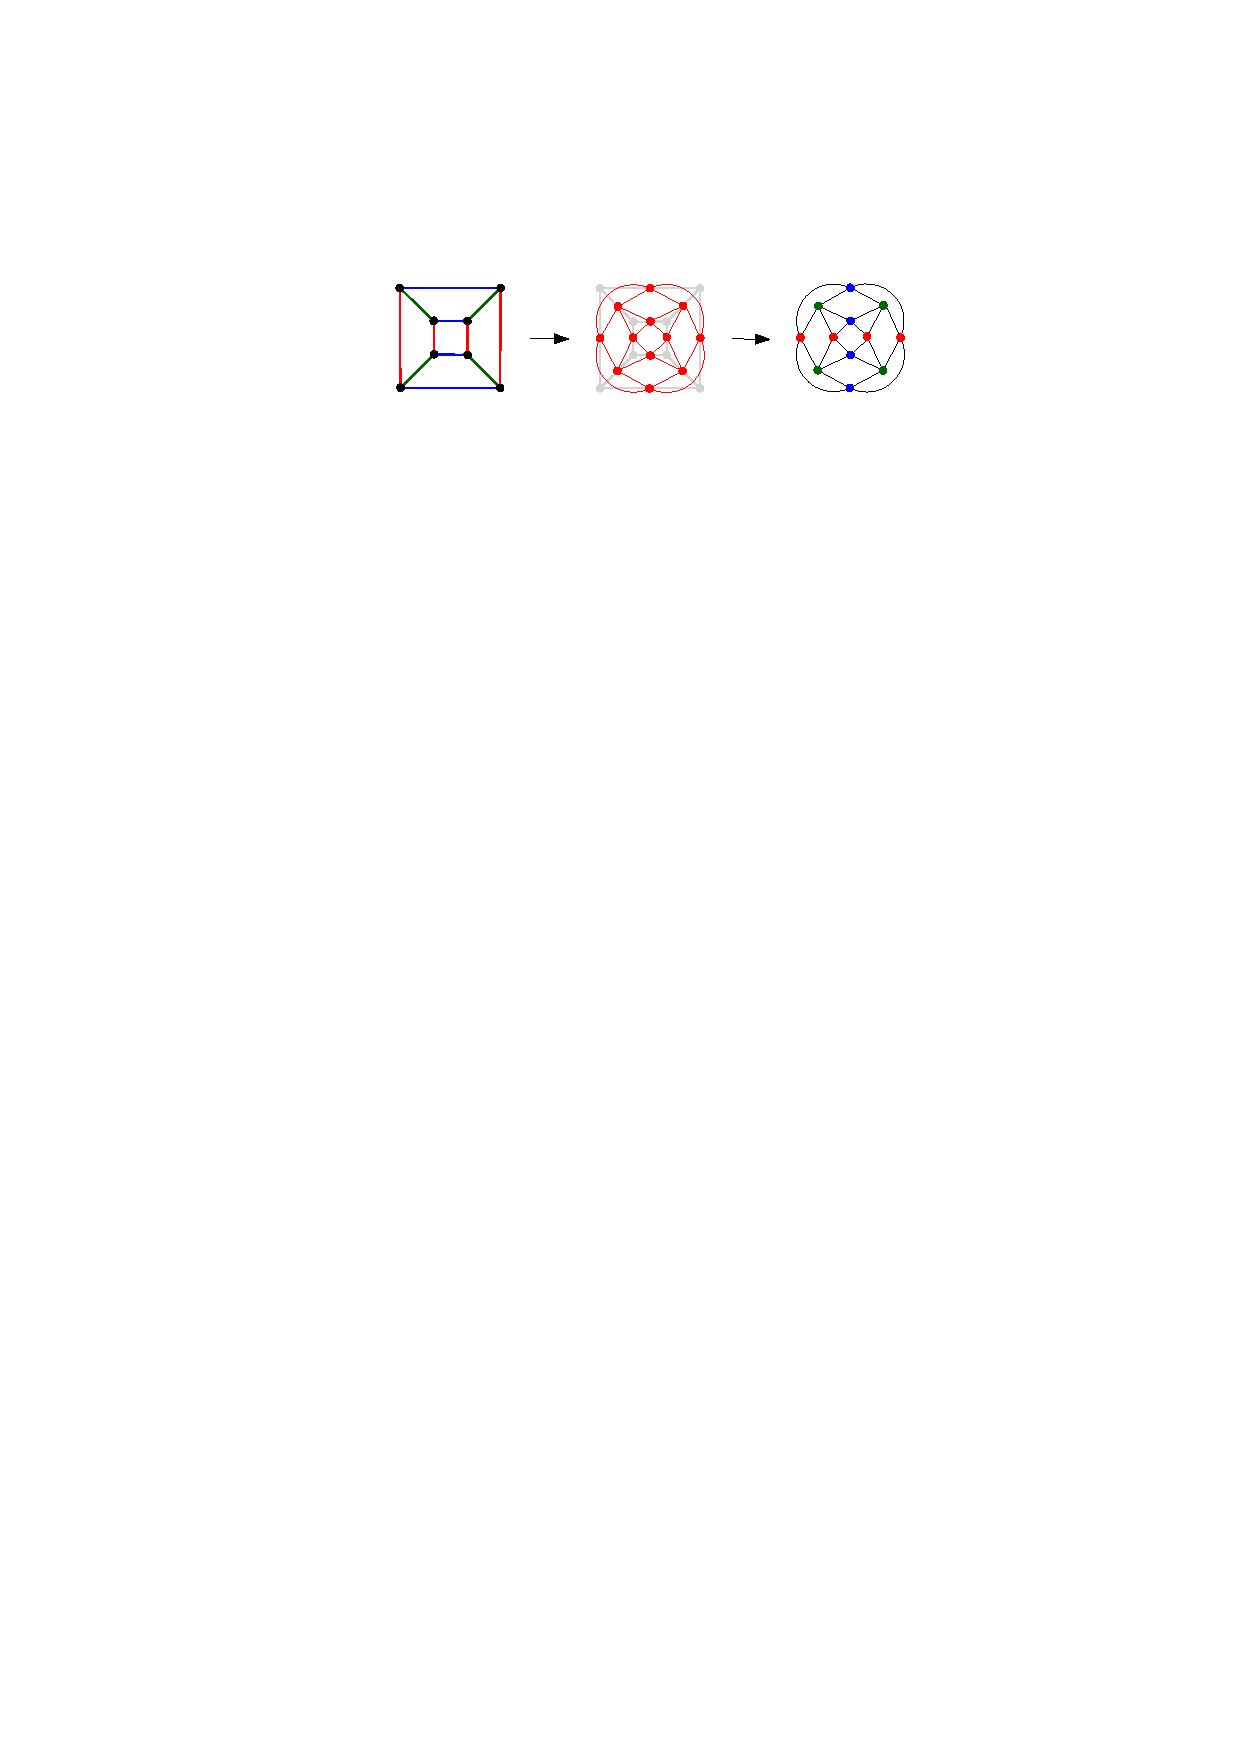
\includegraphics[width=1\textwidth]{../Resources/Figs/cubical_line_graph.pdf}
    \caption{Visualization of conversion from edge coloring to vertex coloring using a line graph}
    \label{fig:cubical_line_graph}
\end{figure}

Note that in Figure~\ref{fig:cubical_line_graph} above, the operation of creating the line graph corresponds to the cube rectification operation. In this particular case, we transformed the graph of a cube into the graph of a cuboctahedron.

\section{Total coloring to vertex coloring}

Intuitively, since total coloring assigns colors to both edges and vertices, it makes sense to use a combination of the original graph and its line graph. However, we cannot simply combine these two graphs by taking the union of their vertex and edge sets and then apply vertex coloring to the resulting graph. The problem is that nothing would prevent us from assigning the same color to an edge and one of its endpoints, since the vertices corresponding to the edge and its endpoint would not be adjacent in the combined graph. This brings us to the so-called \textit{incidence graph}.

\begin{defn}[incidence graph]
    For a graph $G = (V, E)$, we define its \emph{incidence graph} $G_I = (V_I, E_I)$ as follows:
    \begin{enumerate}
        \item $V_I := V \cup E$
        \item $E_I := \{ \{v, e\} : v \in V, e \in E, v \in e \}$
    \end{enumerate}
\end{defn}

Again, note how the definition of $E_I$ corresponds to the coloring rule \ref{eqn:tot_rule}.

\begin{figure}[H]
    \centering
    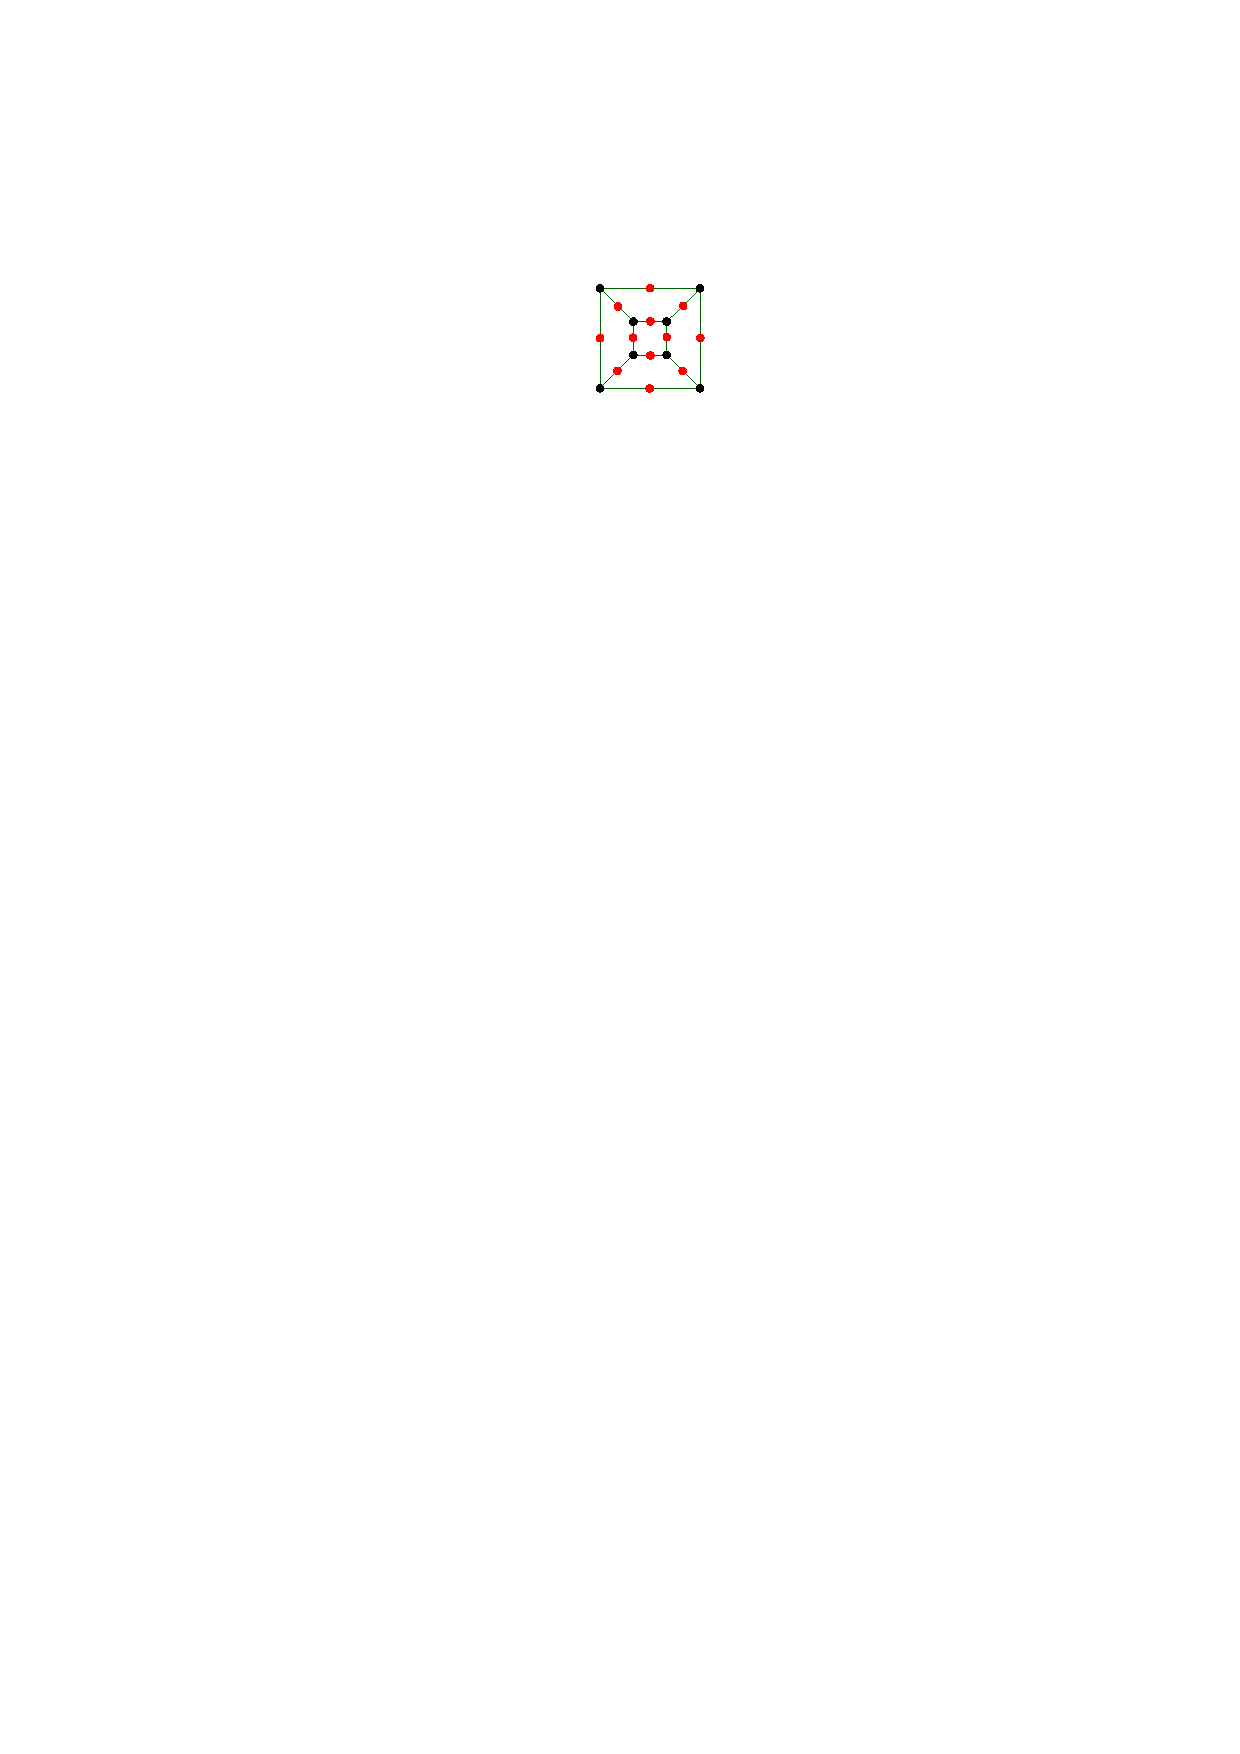
\includegraphics[width=0.2\textwidth]{../Resources/Figs/cubical_incid_graph.pdf}
    \caption{Example of the incidence graph of a cubical graph}
    \label{fig:cubical_incid_graph}
\end{figure}

Now we have all the necessary tools to define a \textit{total graph}, which has the property, that its vertex coloring corresponds exactly to the total coloring of the original graph.

\begin{defn}[total graph]
    Let $G = (V, E)$ be a graph. Let $G_L = (V_L, E_L)$ and $G_I = (V_I, E_I)$ be its line graph and incidence graphs respectively. We define its \emph{total graph} $G_T = (V_T, E_T)$ as follows:
    \begin{enumerate}
        \item $V_T := V_I$
        \item $E_T := E \cup E_L \cup E_I$
    \end{enumerate}
\end{defn}

In natural language, we start with the vertices and edges of the incidence graph. Then, we split the vertices of the incidence graph into two disjoint sets: the set of vertices of the original graph and the set of vertices of the line graph. In the former set, we connect any two vertices that are adjacent in the original graph. In the latter, we do the same using adjacency in the line graph.

\begin{figure}[H]
    \centering
    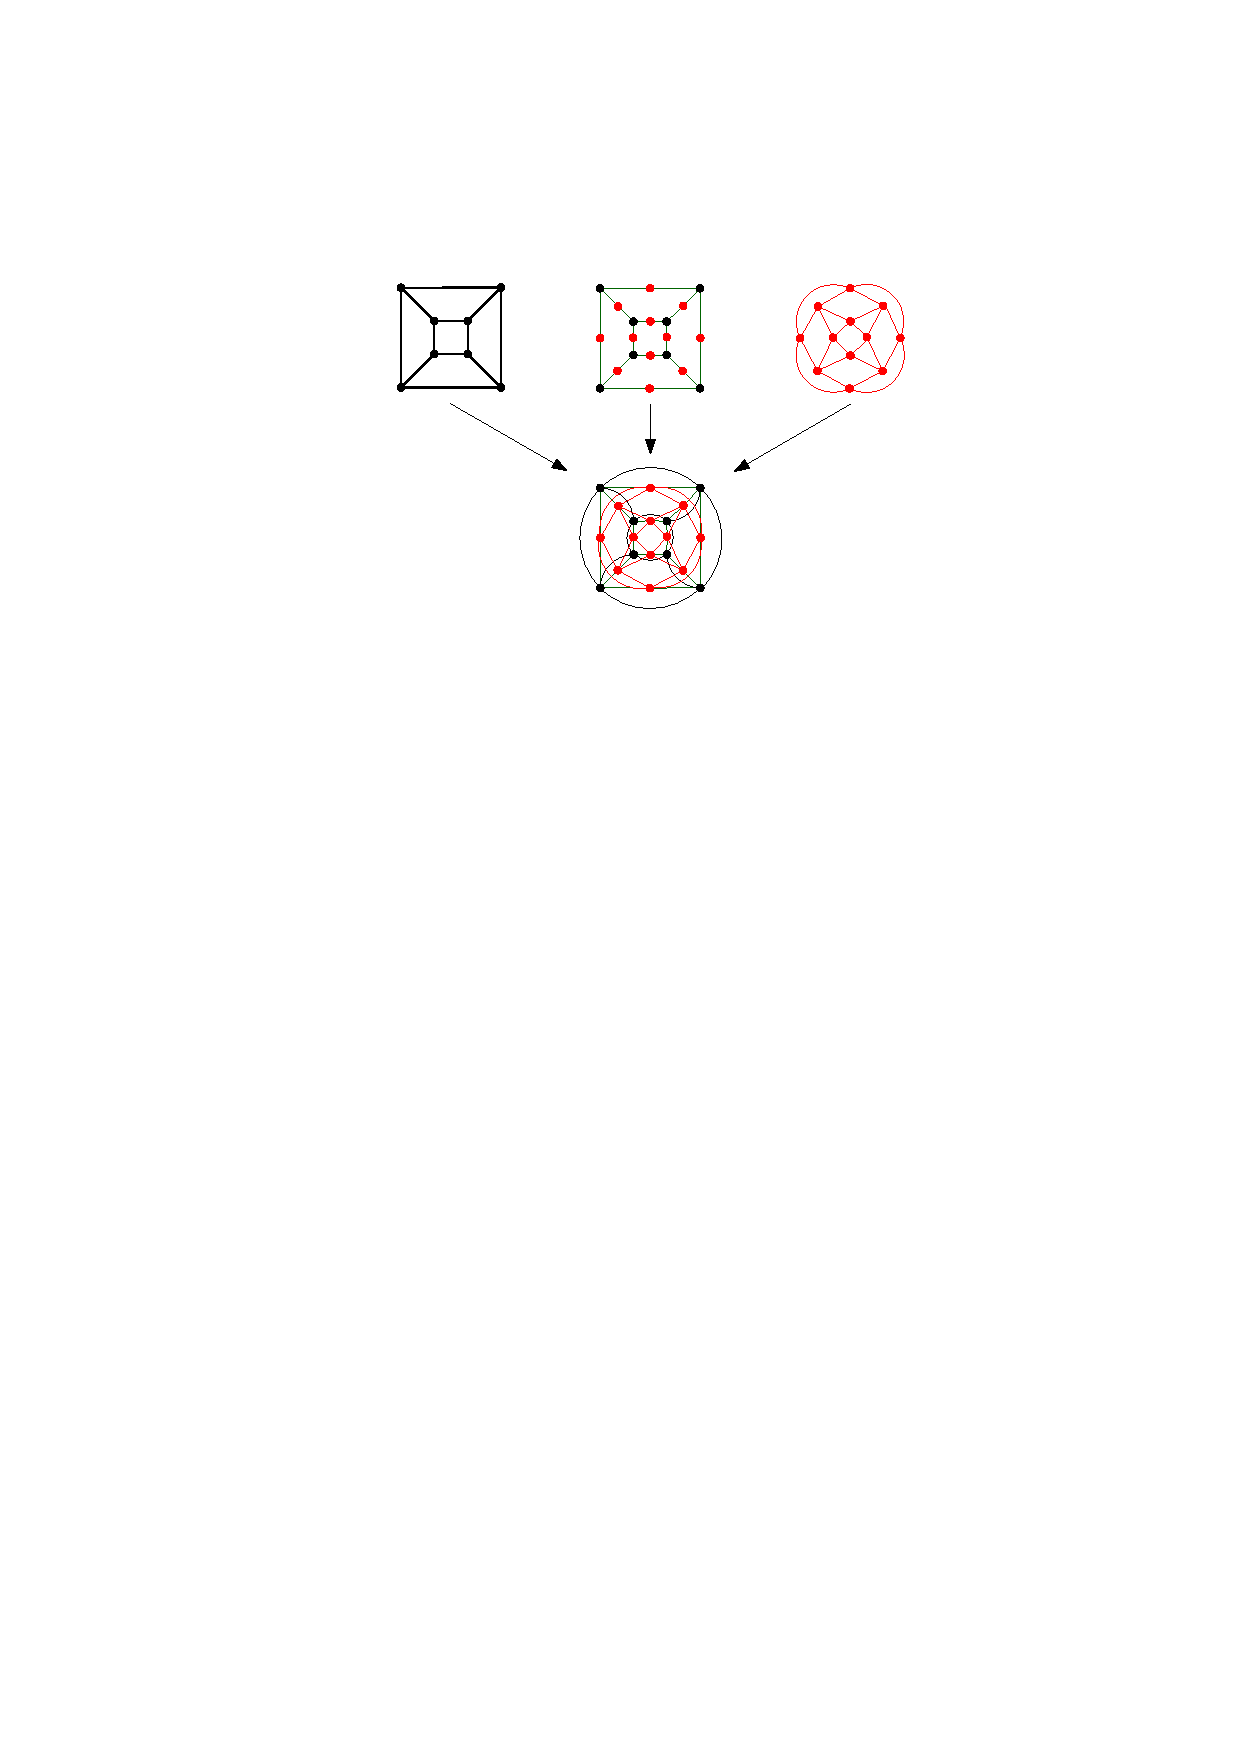
\includegraphics[width=1\textwidth]{../Resources/Figs/cubical_total_graph.pdf}
    \caption{Visualization of total graph construction from the original graph, incidence graph, and line graph.}
    \label{fig:cubical_total_graph}
\end{figure}

\begin{figure}[H]
    \centering
    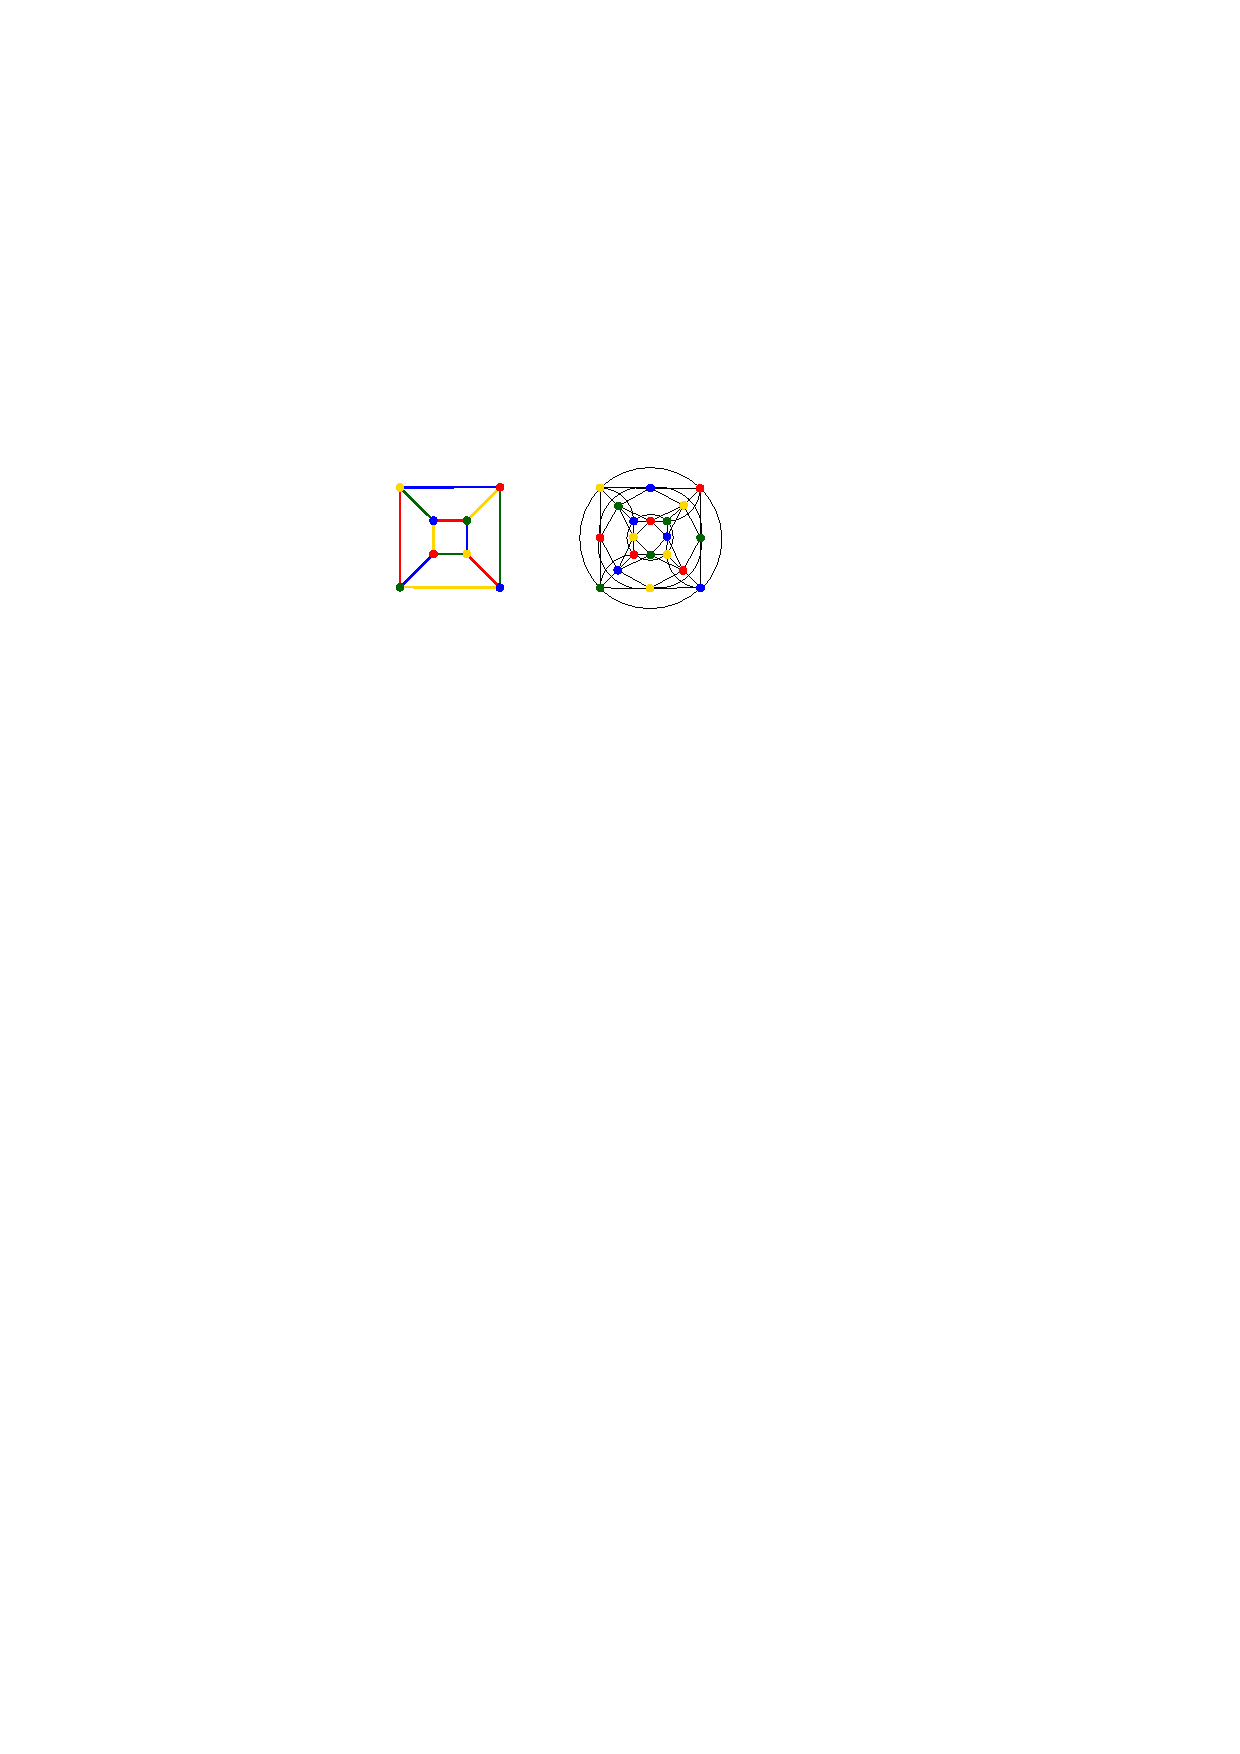
\includegraphics[width=0.6\textwidth]{../Resources/Figs/cubical_tot_g_clring_opt.pdf}
    \caption{Correspondence between the total coloring of the original graph and the vertex coloring of its total graph.}
    \label{fig:cubical_tot_g_clring}
\end{figure}

\section{Face coloring to vertex coloring}

For the conversion from face coloring to vertex coloring, we apply the same idea as when constructing line graphs. However, since the elements being colored are faces rather than edges, we need to encode adjacency of faces into the new graph by adding edges where necessary. The resulting graph is called the \textit{dual graph}.

\begin{defn}[dual graph]
    For a plane graph $G = (V, E, F)$, we define its \emph{dual graph} $G_D = (V_D, E_D)$ as follows:
    \begin{enumerate}
        \item $V_D := F$
        \item $E_D := \{ \{R_1, R_2\} \in \binom{F}{2} : \bnd(R_1) \cap \bnd(R_2) \neq \emptyset \}$
    \end{enumerate}
\end{defn}

\begin{figure}[H]
    \centering
    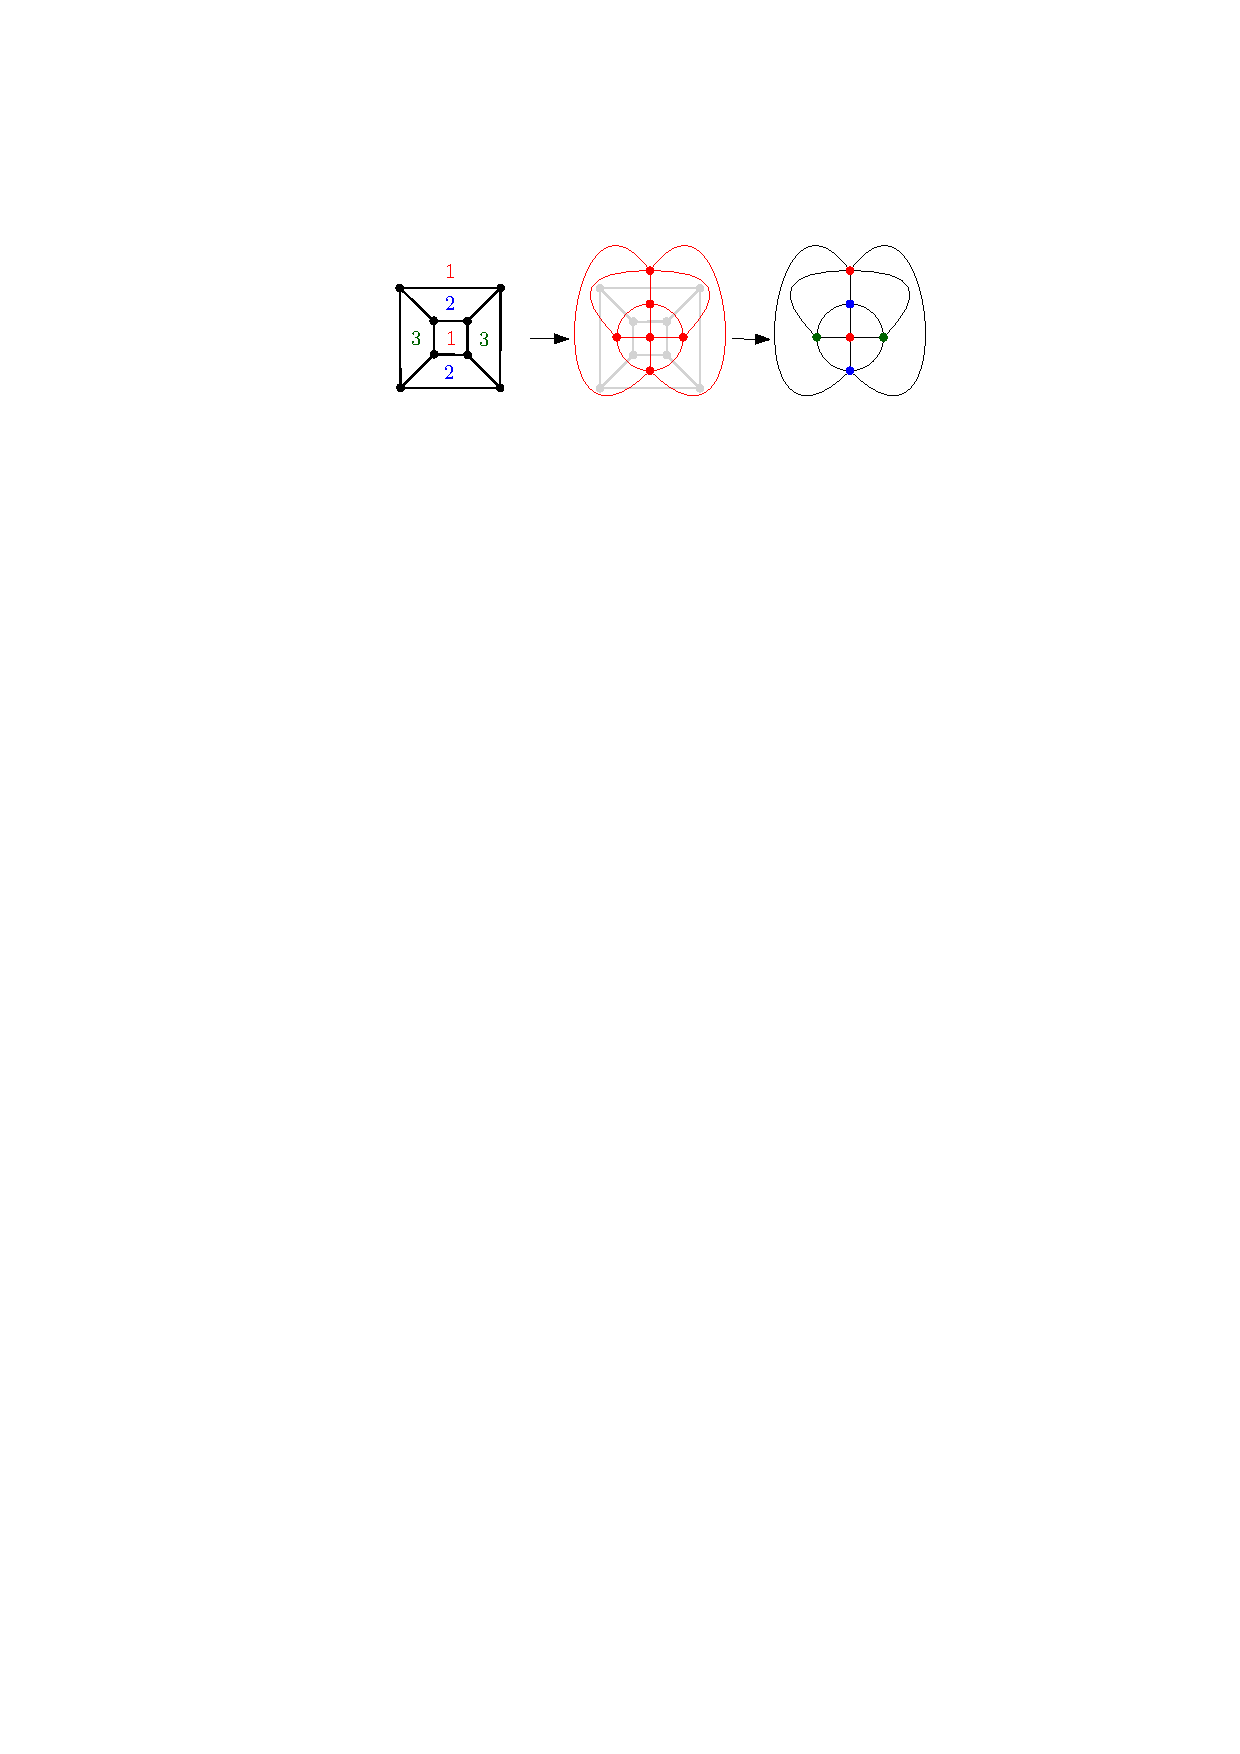
\includegraphics[width=1\textwidth]{../Resources/Figs/cubical_dual_graph.pdf}
    \caption{Visualization of conversion from face coloring to vertex coloring using a dual graph}
    \label{fig:cubical_dual_graph}
\end{figure}